\chapter[Online reprocessing simulation]{Online reprocessing simulation}

\section{Fuel salt processing systems}
Removing specific chemical elements from a molten salt is a complicated task that requires intelligent design (e.g., chemical separations equipment design, fuel salt flows to equipment) and has a considerable economic cost. This section contains \gls{MSBR} chemical processing plant and gas separation system brief overview.

\subsection{Fuel salt chemical processing facility}
All liquid-fueled \gls{MSR} designs involve varying levels of online fuel processing. Minimally, volatile gaseous fission products (e.g. Kr, Xe) escape from the fuel salt during routine reactor operation and must be captured. Additional systems might be used to enhance removal of those elements. Most designs also call for the removal of rare earth metals from the core since these metals act as neutron poisons. Some designs suggest a more complex list of elements to process (figure ~\ref{fig:periodic_tab}), including the temporary removal of protactinium from the salt or other regulation of the actinide inventory in the fuel salt \cite{ahmad_neutronics_2015}.

In the single-fluid \gls{MSBR} considered in this work, thorium, uranium, protactinium, and fission products are all mixed together in a single fluoride salt (FLiBe). Separation of thorium from lanthanide (atomic numbers 57 through 71) fission products is rather challenging because of their chemical similarities. 
\begin{figure}[htp!] % replace 't' with 'b' to 
  \centering
  \vspace{-0.3em}
  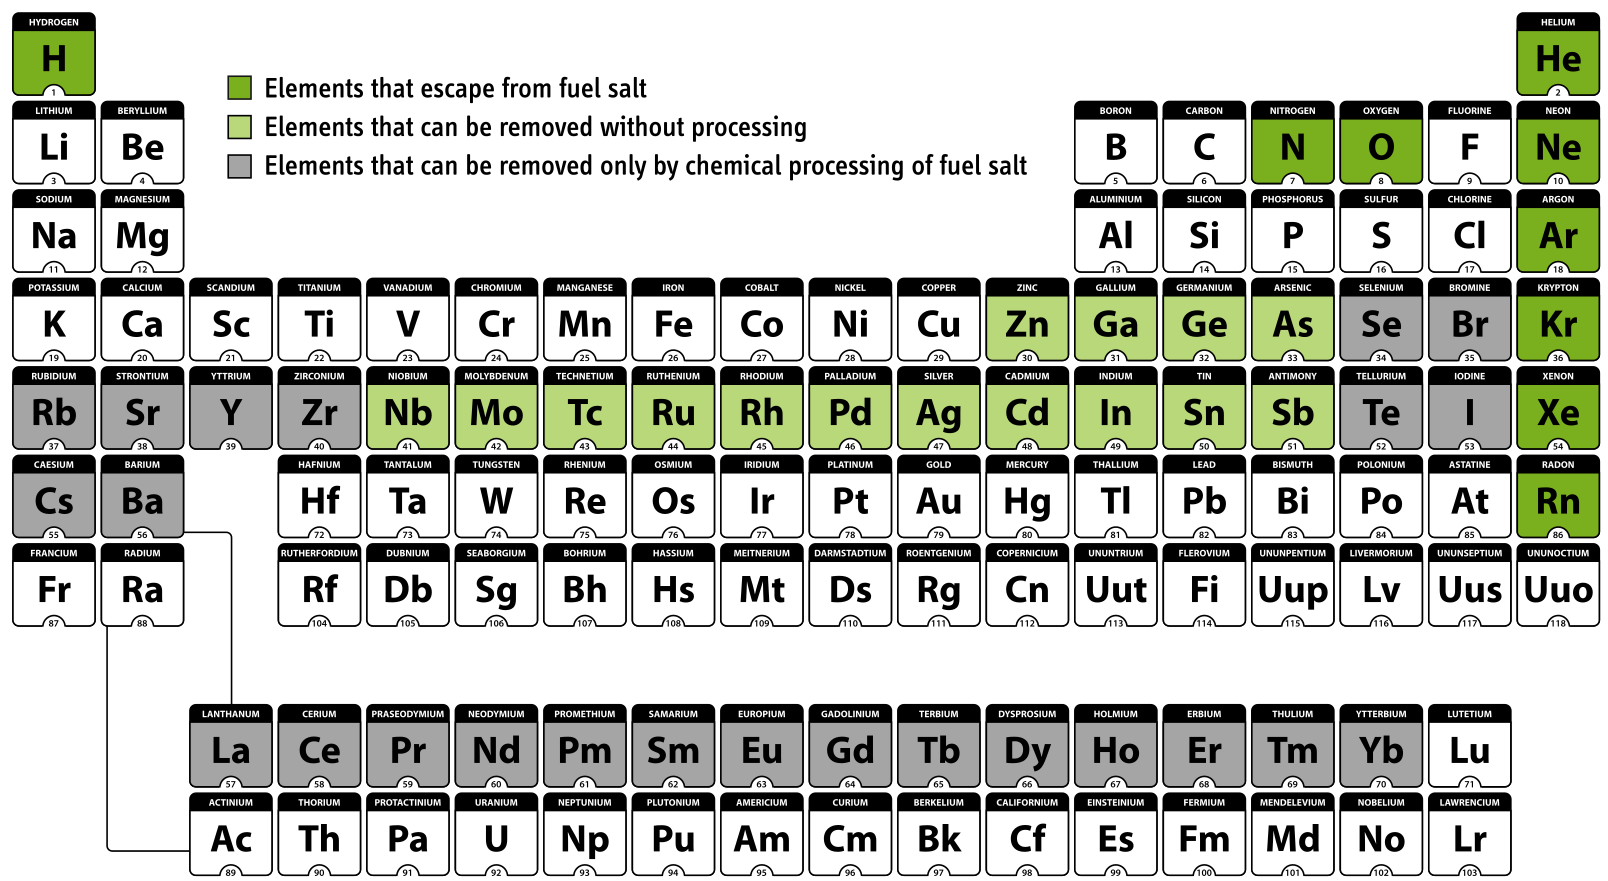
\includegraphics[width=\textwidth]{periodic_map.png}
  \caption{Processing options for \gls{MSR} fuels \cite{ahmad_neutronics_2015}.}
  \vspace{-0.6em}
  \label{fig:periodic_tab}
\end{figure}
\FloatBarrier

The principal scheme of \gls{MSBR} reprocessing facility concept is shown in Figure~\ref{fig:material_flow}. The fuel salt is first temporarily stored for cooling and decay of the shortest lived fission products, then directed to the primary fluorinator, where most of the uranium is removed by fluorination to UF$_6$. After that, the salt is routed to an extraction column where mixture containing metallic bismuth, lithium and thorium as reductants are contacted with the salt. The remaining uranium and protactinium are reductively extracted to the bismuth, leaving a salt that only contains fission products dissolved in carrier salt (base composition of LiF-BeF$_2$-ThF$_4$).The salt then goes through a reduction column where UF$_6$ is reduced to UF$_4$ in the salt, refueling it and preparing it for return to the reactor. Refill BeF$_2$ and ThF$_4$ are also added and all residual bismuth is removed from the salt. After a final cleanup step and valence adjustment, the purified salt returns to the reactor \cite{carter_design_1972,sorensen_one-fluid_2006}.

The bismuth accommodating some uranium and protactinium is routed to a hydrofluorination column where the metallic solutes in the bismuth are oxidized into their fluoride forms in the presence of a decay salt. The decay salt, containing UF$_4$, PaF$_4$, and ThF$_4$ passes into a decay tank where $^{233}$Pa is decaysto $^{233}$U. The uranium generated by protactinium decay is removed through fluorination to UF$_6$ and directed to the reduction column to refuel the purified fuel salt. A hydrofluorinator and a fluorinator can remove approximately \textbf{95\%} of the uranium from the stream.

The fully processed salt, on its way back to the reactor, has uranium added from the protactinium decay tank at the rate required to maintain or adjust the uranium concentration in the reactor (and, consequently, control the reactivity). This is performed by sparging the salt with UF$_6$ and hydrogen to produce UF$_4$ in the salt and HF gas \cite{robertson_conceptual_1971}.

\begin{figure}[htp!] % replace 't' with 'b' to 
  \centering
  \vspace{-0.3em}
  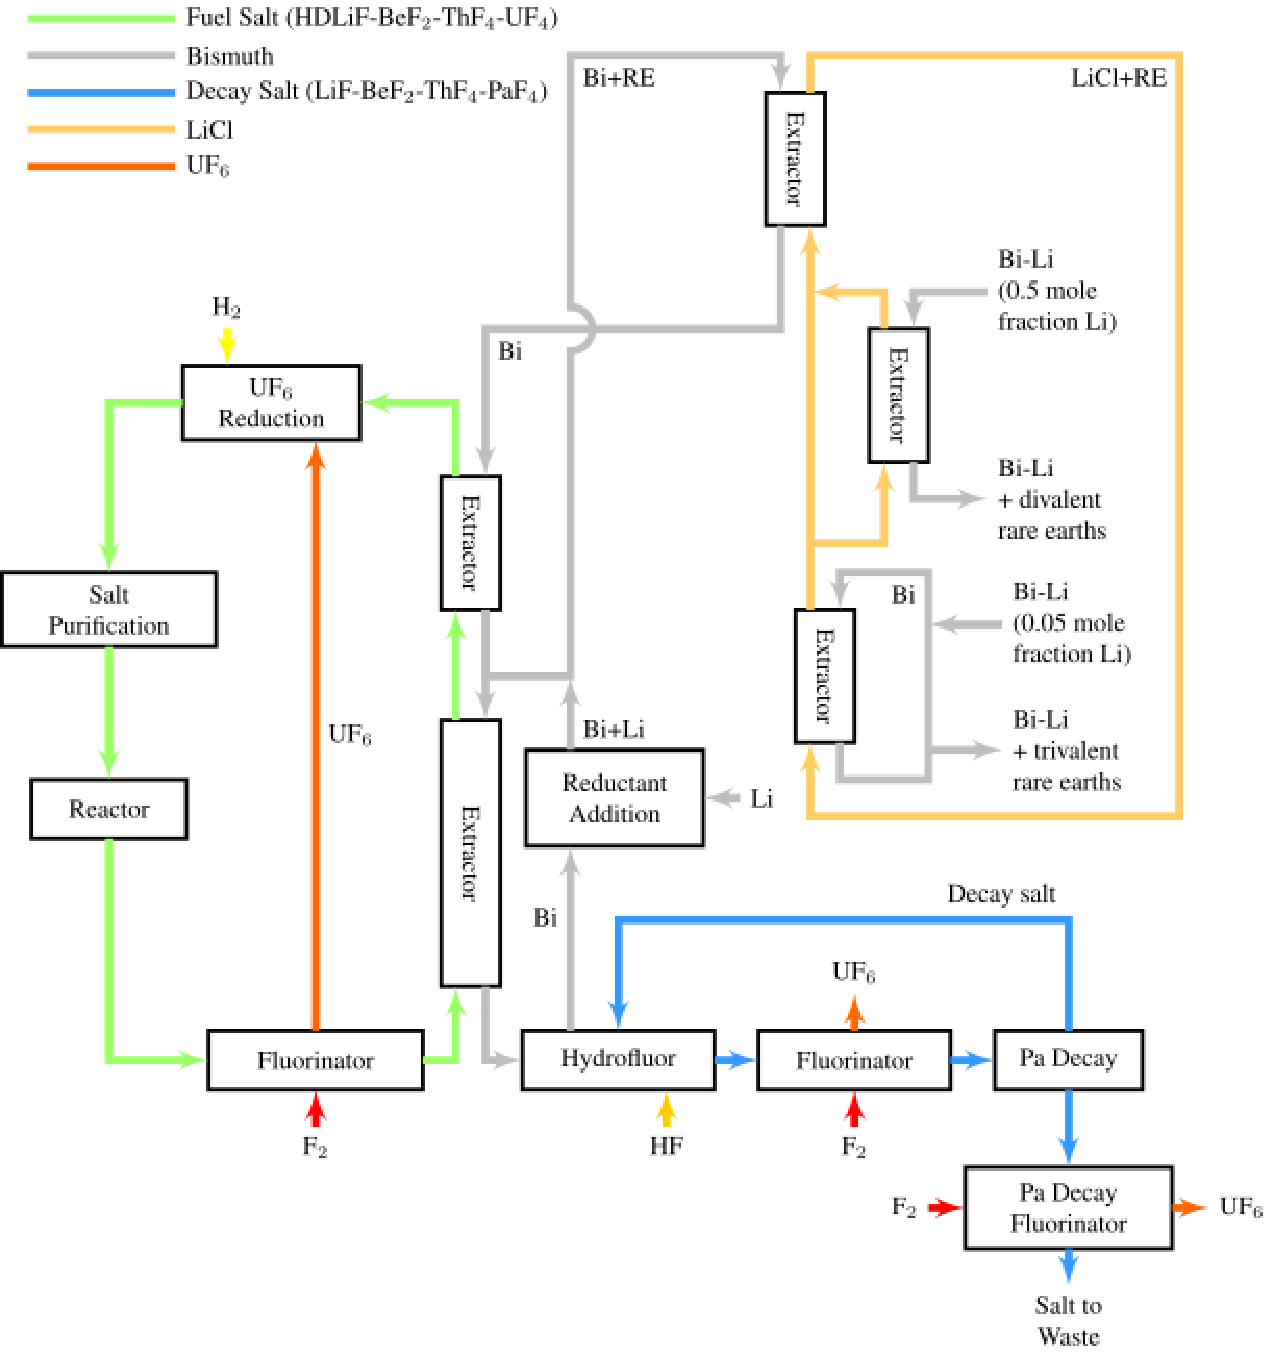
\includegraphics[width=\textwidth]{flowsheet.pdf}
  \caption{Detailed block diagram of chemical processing scheme for single-fluid \gls{MSBR} \cite{robertson_conceptual_1971, sorensen_one-fluid_2006}.}
  \vspace{-0.6em}
  \label{fig:material_flow}
\end{figure}
\FloatBarrier

\subsection{Gas separation system}
Volatile gaseous fission products (e.g. Kr, Xe) must be removed from the fuel salt to avoid reactor poisoning especially during starup and power maneuvering. This is particularly true for $^{135}$Xe, with its very large absorption cross section. Tritium, xenon, and krypton are sparged from the fuel salt by helium introduced in a bypass stream by a bubble generator and subsequently removed by a gas separator. Indeed, noble gases, because of their exceptional insolubility in the salt, will migrate promptly to any gaseous interface available. Because they form ideal-dilute mixture in salt (obey Henry's law), they will migrate in accordance with the conventional laws of mass transfer. If tiny helium bubbles are circulated with the fuel salt, they will absorb xenon and krypton fission products. The fission-product-rich bubbles of helium may then be separated from the salt and discharged to the off-gas system. Xenon migration to the circulating bubbles is in competition with xenon migration to the porous moderator graphite. The graphite is especially of concern because it absorbs xenon and holds it in the core which leads to parasitic neutron absorption. The 0.5\% target value for $^{135}$Xe poison fraction can be achieved when circulating helium bubbles 0.508mm in diameter \cite{robertson_conceptual_1971}. This is accomplished by bypassing 10\% of the fuel salt from the pump discharge through a bubble separator to remove the xenon bubbles and then back into the pump suction, as shown in Figure~\ref{fig:gas_removal_system}. The average residence time of a bubble in the fuel loop would be 10 full cycles.

\begin{figure}[htp!] % replace 't' with 'b' to 
  \centering
  \vspace{-0.3em}
  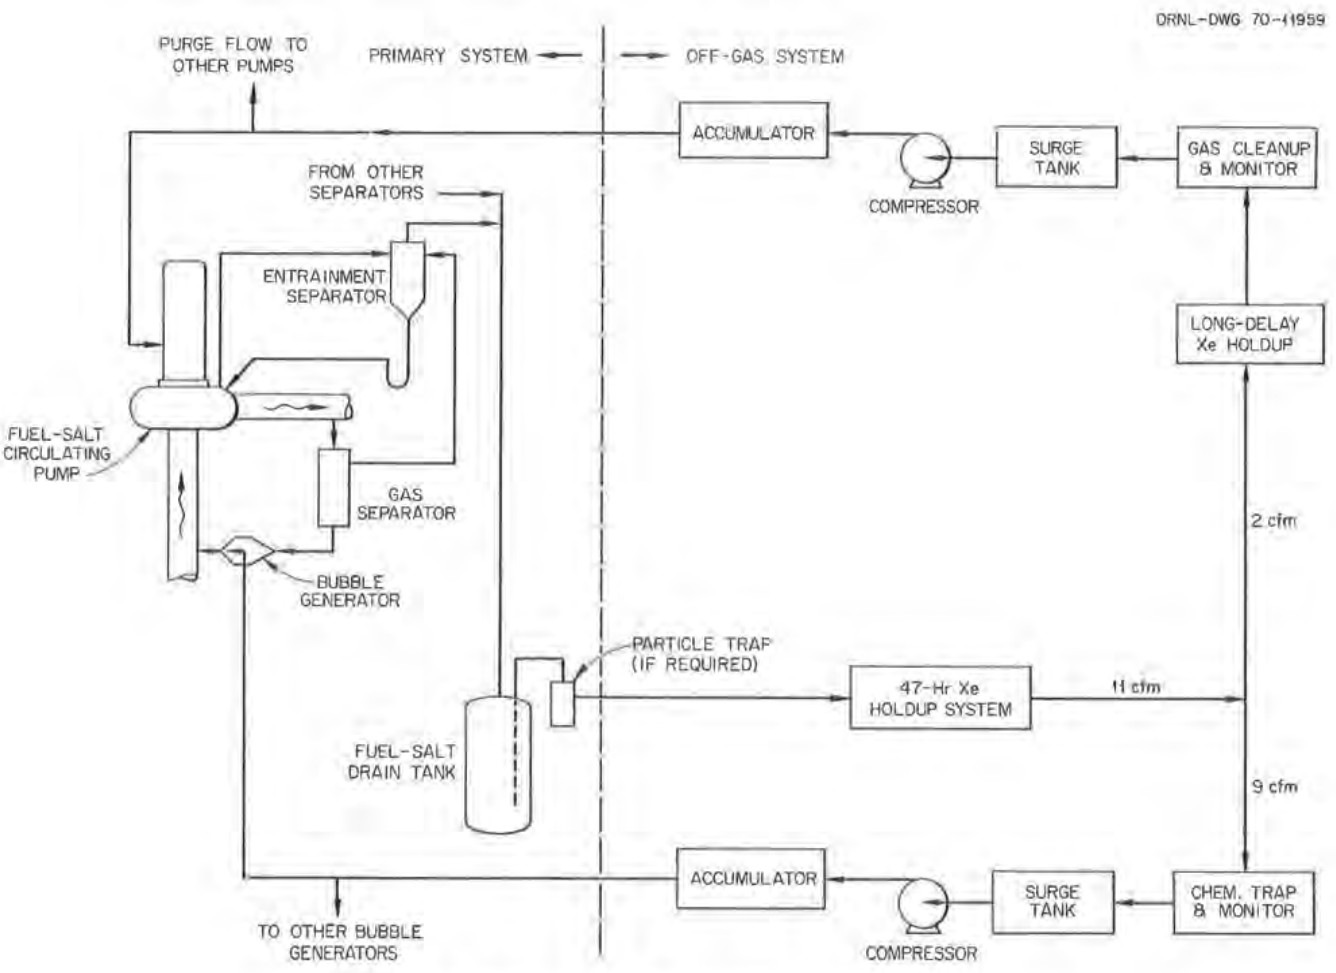
\includegraphics[width=\textwidth]{gas_separation.png}
  \caption{Flow diagram for \gls{MSBR} plant. Green line indicates gas separation and off-gas system \cite{robertson_conceptual_1971}.}
  \vspace{-0.6em}
  \label{fig:gas_removal_system}
\end{figure}
\FloatBarrier
\section{Online reprocessing method}
Modeling liquid-fueled systems with existing neutron transport and depletion tools is challenging because most of these tools are designed for the solid-fueled reactors simulation. The fuel material flows and potential online separations or feeds of specific elements or nuclides are the main challenges of liquid-fueled systems. SaltProc accounts for online feeds and separations using SERPENT 2 neutron transport and burnup capabilities.

\subsection{Online separations and feeds}
The ability to perform online fuel salt reprocessing improves the potential neutronic performance of liquied-fueled reactors. Firstly, it is unnecessary for liquid-fueled reactors to operate with excess reactivity because fissile material is continuously being added into the core. Secondly, continuously removing fission products including strong absorbers (poisons) should significantly improve fuel utilization and decrease parasitic neutron absorption. Finally, neutronic parameters could be adjusted ``on-the-fly" without operational cycle interruption. Nevertheless, removal of each element from the liquid fuel salt presents a unique challenge in terms of storage and disposal of the separated materials.

To take into account online reprocessing, two potential approaches can be implemented. One is a batch-wise approach where material is moved into or from the core at specific time intervals (batch). This approach assumes that material accumulation in the core during the time between separations or feeds does not affect reactor physics. This method requires the simulation to stop, modify the fuel composition, and restart. This approach was implemented in a ChemTriton script \cite{powers_new_2013} which has been developed by T.J.Harrision, \gls{ORNL}, and actively using for online reprocessing simulation with SCALE/TRITON \cite{bowman_scale_2011} and Shift \cite{pandya_implementation_2016}. 

Another approach approximates more continuous reprocessing where material is separated from (or added into) the core at all times to simulate true continuous online reprocessing. This method is more difficult because it requires adding a term to the Bateman equations. In SCALE/TRITON, ORIGEN \cite{gauld_isotopic_2011} solves a set of Bateman equations using one-group averaged fluxes and cross-sections obtained from a transport calculation. Bateman equations that describe the rate of change of the isotopes due to neutron induced reactions and decay
processes could be written in this form \cite{aufiero_extended_2013}:

\begin{align}
        \frac{dN_i}{dt} &= \bar{\Phi}\sum\limits_{j}N_{j}\sigma_{j \rightarrow 		i} - \bar{\Phi}\sum\limits_{j}N_{i}\sigma_{i \rightarrow j} + \sum					\limits_{j}	N_{j}\lambda_{j}b_{j \rightarrow i} - N_{i}\lambda_{i}
\label{eq:bateman}
	\intertext{where} 
	N_i &= \mbox{number density of isotope i} \\
	N_j &= \mbox{number density of isotope j} \\
	\bar{\Phi} &= \mbox {average in the space and energy neutron flux} \\
	\sigma_{j \rightarrow i} &= \mbox{microscopic one-group transmutation cross section} \\
	\lambda_i &= \mbox{decay constant of nuclide i} \\
	\lambda_j &= \mbox{decay constant of nuclide j} \\
	b_{j \to i} &= \mbox{branching fractions of radioactive decay from nuclide j}
\end{align}

The four terms on the right-hand side of the equation represent (1) the production rate of nuclide $i$ from irradiation, (2) the loss rate of nuclide $i$ due to irradiation, (3) the decay rate of nuclide $j$ into nuclide $i$, and (4) the loss rate of nuclide $i$ due to decay. Mentioned earlier deterministic codes SCALE/TRITON and Monte Carlo codes MCNP, Shift, KENO-VI do not support non-zero removal or feeds rates for depletion simulations.

Online fuel reprocessing can be explicitly introduced in the system of equations by adding effective decay and transmutation terms for the various nuclides. During fuel composition evolution calculations, the total mass fraction of thorium fluoride is kept constant at 12\%. For this purpose, $^{233}$Th isotope is replaced with the fresh $^{232}$Th feed material. This could be achieved with an additional gain term on the right-hand side of the Bateman equation:
\begin{align*}
\bar{\Phi}\sum\limits_{k=^{232}Th}N_{k}\sigma_{k,c}
\end{align*}
where $\sigma_{k,c}$ is the one-group capture cross section of thorium-232.

The removal of fission products and protactinium is achieved by adding an explicit decay term to the Bateman equations. For the generic fission product, l, loss term can be added:
\begin{align*}
- N_{l}\lambda_{l,reproc}
\end{align*}
where $\lambda_{l,reproc}$ is the effective removal time constant of the particular chemical species. This approach was recently implemented as a purpose-made extension within the continuous-energy Monte Carlo reactor physics and burn-up code SERPENT \cite{aufiero_extended_2013} but it is not currently available for external users.

I have developed the SaltProc Python package \cite{andrei_rykhlevskii_arfc/saltproc:_2018}, implementing batch-wise approach coupled with the SERPENT 2 burnup routine. A high-fidelity full-core \gls{MSBR} model serves as a basis for the online reprocessing simulation described in this thesis. 

\subsection{Fuel material flows}
The $^{232}$Th in the fuel absorbs thermal neutrons and produces $^{233}$Pa which then decays into the fissile $^{233}$U. Furthermore, the \gls{MSBR} design requires online reprocessing to remove all poisons (e.g. $^{135}$Xe), noble metals, and gases (e.g. $^{75}$Se, $^{85}$Kr) every 20 seconds. Protactinium presents a challenge, since it has a large absorption cross section in the thermal energy spectrum. Accordingly, $^{233}$Pa is continuously removed from the fuel salt into a protactinium decay tank to allow $^{233}$Pa to decay to $^{233}$U without poisoning the reactor. The reactor reprocessing system is designed to separate $^{233}$Pa from the molten-salt fuel over 3 days, hold it while $^{233}$Pa decays into $^{233}$U, and return it back to the primary loop. This feature allows the reactor to avoid neutron losses to protactinium, keeps fission products to a very low level, and increases the efficiency of $^{233}$U breeding. Table~\ref{tab:reprocessing_list} summarizes full list of nuclides and the cycle times used for modeling salt treatment and separations \cite{robertson_conceptual_1971}. 

%%%%%%%%%%%%%%%%%%%%%%%%%%%%%%%%%%%%%%%%
\begin{table}[ht!]
        \centering
        \caption{The effective cycle times for protactinium and fission products removal (reproduced from \cite{robertson_conceptual_1971}).}
        \begin{tabular}{|m{0.25\textwidth} | m{0.45\textwidth}|m{0.16\textwidth}|}
        \hline 
        %\begin{tabularx}{\linewidth}{l X} \toprule 
        Processing group & \qquad\qquad\qquad Nuclides & Cycle time (at full power) \\ [5pt] \hline 
        Rare earths & Y, La, Ce, Pr, Nd, Pm, Sm, Gd & 50 days \\ [5pt] \hline 
        \qquad & Eu & 500 days \\ [5pt] \hline
        Noble metals & Se, Nb, Mo, Tc, Ru, Rh, Pd, Ag, Sb, Te & 20 sec \\ [5pt] \hline
        Seminoble metals & Zr, Cd, In, Sn & 200 days \\ [5pt] \hline
        Gases & Kr, Xe & 20 sec \\ [5pt] \hline
        Volatile fluorides & Br, I & 60 days \\ [5pt] \hline
        Discard & Rb, Sr, Cs, Ba & 3435 days \\ [5pt] \hline
        Salt discard & Th, Li, Be, F & 3435 days \\ [5pt] \hline
        Protactinium & $^{233}$Pa & 3 days \\ [5pt] \hline
        Higher nuclides & $^{237}$Np, $^{242}$Pu & 16 years \\ [5pt] \hline
        \end{tabular}
        %\footnotetext{Chemical processing plant and gas separation system removing chemical elements (not isotopes) only. Isotopes instead of elements listed because other isotopes are short-lived and might be ignored.}
        \label{tab:reprocessing_list}
          \vspace{-0.9em}
\end{table}
Since removal rates vary among nuclides in this reactor concept, the built-in SERPENT 2 reprocessing subroutine is unable to capture the desired reprocessing strategy. The removal rates also dictate the necessary resolution of depletion calculations. If the depletion time intervals are very short, an enormous number of depletion steps are required to obtain the equilibrium composition. On the other hand, if the depletion  calculation time interval is too long, the impact of short-lived fission products is not captured. To compromise, the time interval for depletion calculations in this model was selected as 3 days to correlate with the removal interval of $^{233}$Pa and $^{232}$Th was continuously added to maintain the initial mass fraction of $^{232}$Th.

\subsection{Simplifying assumptions}
The main goal of the present study is to identify the effects adjusting the fuel salt composition, and find equilibrium performance of a thorium \gls{MSBR} fuel cycle. To highlight these effects and simplify the analysis, several assumptions have been made.

First of all, thorium loading during operation was held constant and equal to initial thorium loading (i.e. $m_{Th}(t)=m_{Th}(0)$) with a variable feed rate (in kg/day) of fresh thorium. Because thorium is a fertile material with relatively high absorption cross section, this has important impacts on reactor physics, including negatively impacting reactivity and skewing the fuel-to-moderator ratio which makes neutron energy spectrum harder. While a reduction in the thorium loading reduces the amount of initial fissile material required to achieve criticality, the breeding rate of $^{233}$U should be sufficient to maintain the core critical during operation.

The solubility of heavy metals is a known problem for \glspl{MSR} but it is fundamentally dependent on the type of carrier salt. For this work, solubility limits for uranium were neglected because the molar fraction of UF$_4$ was negligible for the accuracy desired in this work. In addition, this work assumed that addition or removal of soluble material (e.g. UF$_4$) has a small influence on the fuel salt volume, this volume change is not treated here.

Figure~\ref{fig:th_cycle} from Chapter 2 demonstrates that transformation from $^{232}$Th to $^{233}$U is slow process because $^{233}$Pa $\beta$-decay has half-life 27.4 days. Thus, approximately 90 days needed to decay 90\% of $^{233}$Pa to $^{233}$U. Figure~\ref{fig:pa_isolation} shows how protactinium is separated from the fuel salt reprocessing flow. Therefore, if protactinium decay tank is empty at the moment of reactor startup, then the expected fissile material stream would appear only after a few months of reactor operation at full power. To avoid time-dependent feed rate for $^{233}$UF$_4$ it is assumed that the protactinium decay tank initially contain some amount of $^{233}$UF$_4$, and the rate of fissile material flow from the tank to the core is set equal to the $^{233}$Pa removal rate. Moreover, simulated cycle time at full power was set to 20 years ($\approx$ 7300 days). Finally, 100\% reprocessing separation efficiency was assumed.

\begin{figure}[hbp!] % replace 't' with 'b' to 
  \centering
  \vspace{-0.3em}
  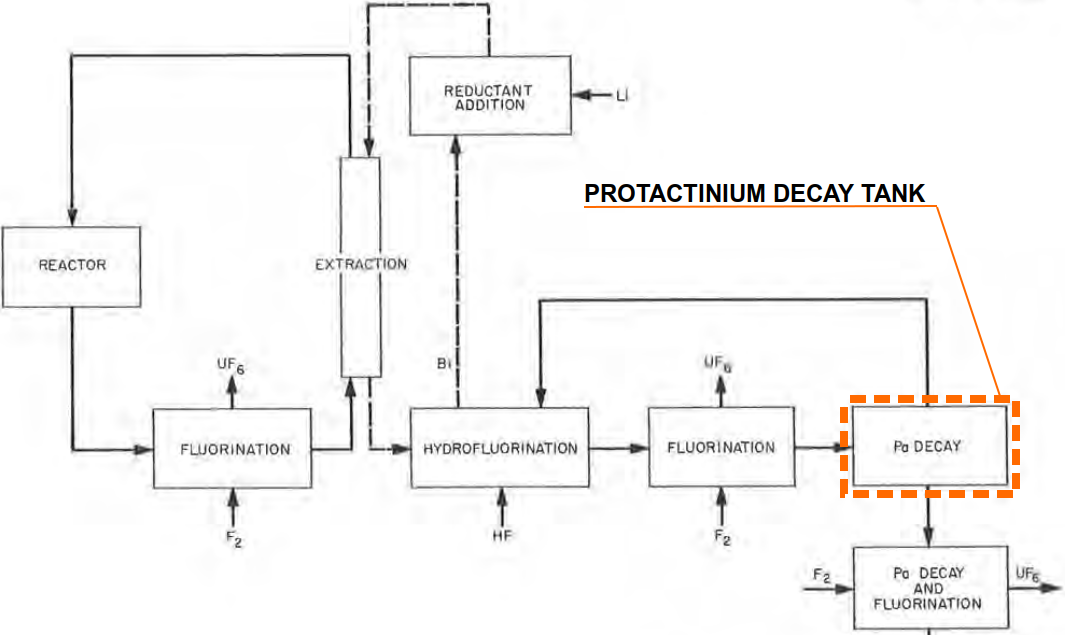
\includegraphics[width=\textwidth]{pa_isolation.png}
  \caption{Protactinium isolation with uranium removal by fluorination \cite{robertson_conceptual_1971}.}
  \vspace{-1.6em}
  \label{fig:pa_isolation}
\end{figure}
\FloatBarrier

The thermal fission of a $^{233}$U in fluoride salts oxidizes the salt. This happens because the uranium nucleus balances the charge of four fluorine ions in the salt (e.g. $^{233}$UF$_4$), but fission products tend to not bind to all the four fluorines released after the uranium fissions. Figure~\ref{fig:excess_fluorine} demonstates an example of an oxidative fission reaction. This excess of fluorine must be compensated, otherwise chemical reactions harmful to reactor components would occur \cite{ridley_method_2017}. In this study, fission-driven salt oxidation is ignored.

\begin{figure}[htp!] % replace 't' with 'b' to 
  \centering
  \vspace{-0.3em}
  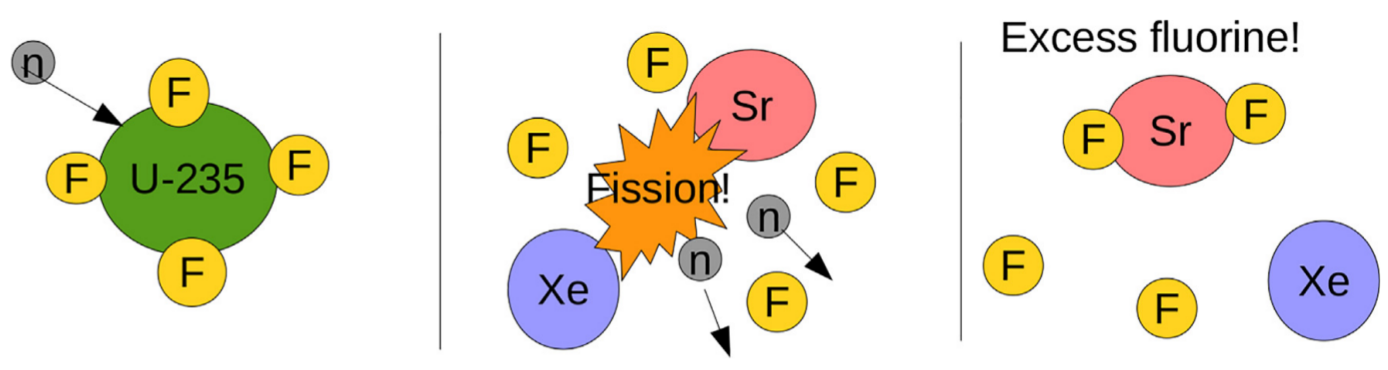
\includegraphics[width=0.8\textwidth]{excess_fluorine.png}
  \caption{Process of production an excess of fluorine due to fission of a $^{233}$U in fluoride salts \cite{ridley_method_2017}.}
  \vspace{-1.0em}
  \label{fig:excess_fluorine}
\end{figure}
\FloatBarrier

Finally, for this study, equilibrium is defined as when $k_{eff}$ and the $^{233}$U concentration in the fuel salt vary less than one percent over several months. 

\section{Python code description}
The objectives for the SaltProc tool were to expand SERPENT 2 burn-up capabilities for modeling liquid-fueled \gls{MSR} and provide an open-source tool for the simulation of reactors where material is removed or added at any time during fuel irradiation. The Python 2.7 packages uses HDF5 \cite{the_hdf_group_hierarchical_1997} to store data and the Nuclear Engineering Toolkit - PyNE \cite{scopatz_pyne:_2012} for SERPENT output file parsing. As was discussed earlier, SaltProc maintains the iterative semi-continuous approach to simulate continuous feeds and removals.

The tool structure and capabilities are similar to ChemTriton tool for SCALE developed in \gls{ORNL} \cite{powers_new_2013}. SaltProc is coupled with Monte Carlo SERPENT 2 software which allows to simulate online reprocessing for irregular full-core geometry with high level of fidelity.  The primary function of SaltProc is to manage material mixtures while SERPENT 2 performs most of the computationally heavy work, namely neutron transport and burnup calculations. Each material stream represents a fluid in the core design and has specific parameters (e.g. isotopic composition, reprocessing interval, mass rate, removal efficacy, etc). In addition, SaltProc provides a set of functions for each stream: read and write isotopic data in/from database, separate out specific isotopes from stream with defined efficiency, feed in specific isotopes to stream, and maintain constant number density of specific nuclide in the core. These attributes and functions are crucial to simulate the operation of a complex, multi-zone, multi-fluid \gls{MSR} and are universal enough for myriad reactor systems.

Figure~\ref{fig:saltproc_flow} demonstrates the  online reprocessing simulation algorithm coupling SaltProc and SERPENT 2. To perform depletion step, SaltProc reads an external SERPENT 2 template file which must be defined by the user. This file contains input cards with data such as geometry, moderator and construction materials isotopic composition, neutron population, criticality cycles, total heating power, and boundary conditions. After the depletion calculation completes, SaltProc reads the burned fuel composition file into memory and stores it in an HDF5 database. SaltProc only knows the number density and isotopic composition of a given fuel stream which provides the tool with the flexibility to model any geometry: an infinite medium, a unit cell, a multi-zone simplified assembly, or a full-core. In some applications the simple single-cell is sufficient to get accurate results for depletion calculations. However, some applications require more geometric fidelity and therefore rely on this flexibility in SaltProc.

SaltProc can manage as many fuel streams as desired. It also may work with multiple depletion materials. At the end of a each depletion step, SaltProc reads the depleted compositions and tracks each material stream individually. Following this, it applies chemical reprocessing functions to fuel stream vectors. These vectors then form a matrix which SaltProc stores in an HDF5 database and prints into the SERPENT 2 composition file for the next depletion calculation.

Liquid-fueled \gls{MSBR} design in this thesis focuses on the state of the core at an equilibrium condition, after fission products have built up in the fuel salt during years if operation. Isotopic composition of the fuel salt continues change slightly even after decades of operation, but the dominant nuclides that have significant impact to the neutronic behavior tend to reach an equilibrium concentration (e.g., vary less than 1\% over several years). In contrast, from the startup of an \gls{MSBR} until the equilibrium condition, the fuel salt composition undergoes significant changes (e.g., changes in fission products, minor actinides, and fissile materials number density). During this period, the material feeds and removals should be optimized for the fastest \gls{MSBR} transition to an equilibrium state. A faster transition simplifies the reactor operation because, at equilibrium, the fissile and fertile feed rates, fission product removal rates, and corresponding core safety parameters are constant in time.

\begin{figure}[htp!] % replace 't' with 'b' to 
  \centering
  \vspace{-0.3em}
  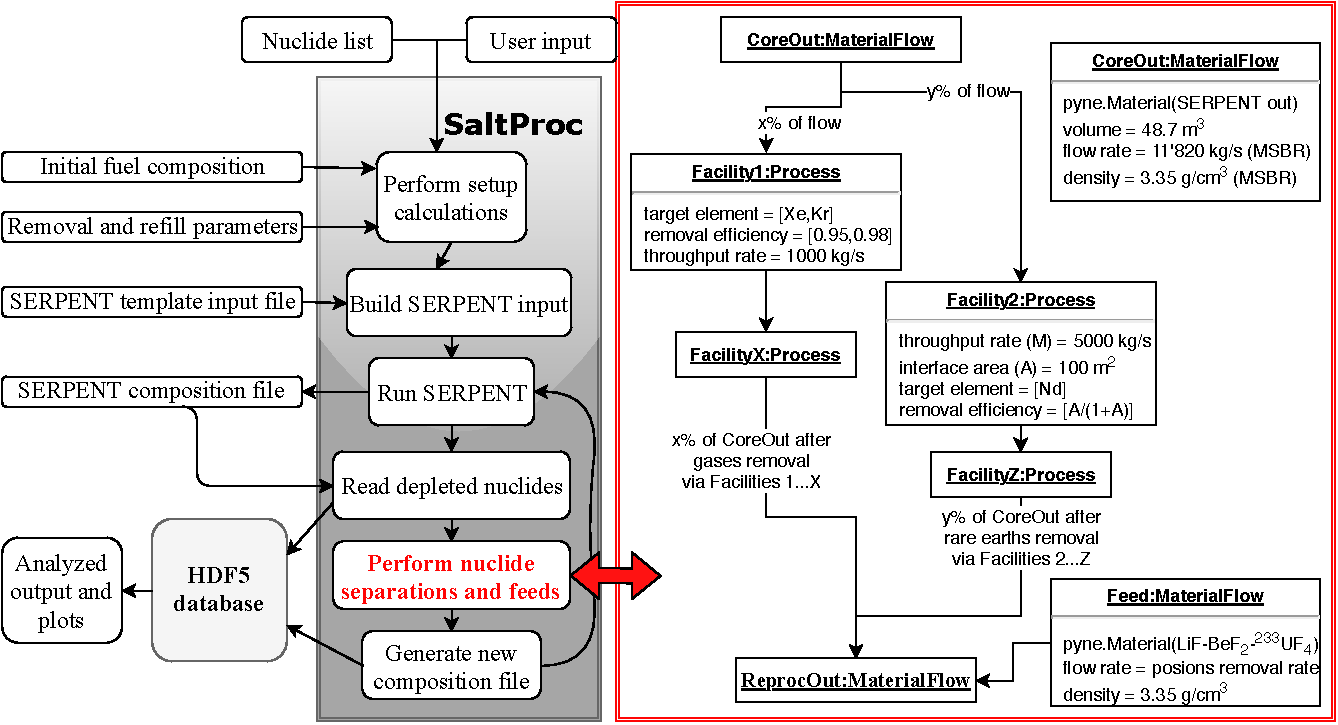
\includegraphics[width=\textwidth]{saltproc_flowchart.pdf}
  \caption{Flow chart for the Saltproc python-based tools.}
  \vspace{-1.0em}
  \label{fig:saltproc_flow}
\end{figure}
\FloatBarrier

In addition, SaltProc is able to define time-dependent material feed and removal rates to investigate the their impacts. These rates need not be constant in SaltProc. They can be defined as piecewise functions or set to respond conditions in the core. For instance, SaltProc might increase the fissile material feeding rate if the effective multiplication factor, $k_{eff}$, falls below a specific limit (e.g., 1.002). 
%Moreover, it could be useful to keep fissile material number density in the %core approximately constant to accumulated excess of $^{233}$U into the %protactinium decay tank. 
These capabilities allow SaltProc to analyze fuel cycle of a generic liquid-fueled \gls{MSR}. In summary, the development approach of SaltProc focused on producing a generic and flexible tool to give the SERPENT 2 Monte Carlo code the ability to conduct advanced fuel cycle analysis as well as simulate a myriad of online refueled systems.
